\documentclass[10pt,twocolumn,letterpaper]{article}
\usepackage[pagenumbers]{cvpr}

\usepackage{booktabs}
\usepackage{multirow}
\usepackage{amsmath}
\usepackage{tikz}
\usetikzlibrary{positioning,arrows.meta,calc}

\definecolor{cvprblue}{rgb}{0.21,0.49,0.74}
\usepackage[breaklinks,colorlinks,allcolors=cvprblue]{hyperref}

\def\confName{CVPR}
\def\confYear{2027}


\title{Where Does CLIP Lose Left and Right?\\
\large Diagnosing the failure and reading it out from patch features}

\author{Seojin Lee\\
Sungshin Women's University\\
{\tt\small \href{https://github.com/SeojinLee06/clip-left-right}{github.com/SeojinLee06/clip-left-right}}
}

\begin{document}
\maketitle

%%%%%%%%%%%%%%%%%%%%%%%%%%%%%%%%%%%%%%%%%%%%%%%%%%%%%%%%%%%%%%%%%%%%%%%%%
\begin{abstract}
CLIP scores ``a mug to the left of a table'' and ``a mug to the right of a table'' almost identically, and What'sUp~\cite{kamath2023whatsup} reports that fine-tuning with left/right-swapped captions does not fix this.
I first confirm this on a 2-way left/right task: text fine-tuning with swapped-caption negatives, with the mirrored image as a matched positive, and with the last image block unfrozen, all stay at chance (49--51\%).
I then ask \emph{where} the information is lost.
A linear probe on CLIP's pooled image vector reaches only 59--62\% on unseen object pairs, and for every test caption the text encoder places its left/right swap closer than a caption with a different subject.
A control that removes CLIP's word bias with the mirrored image leaves accuracy at chance, so bias alone is not the problem.
Before pooling, however, each patch still has a position.
Matching patch features to the two object names and comparing their mean horizontal position, without any training, raises accuracy from about 50\% to 74.3/82.5\% on What'sUp~A, 99.5/100\% on What'sUp~B and 82--90\% on COCO-spatial (ViT-B/32 / ViT-L/14).
The patch read-out itself follows MaskCLIP~\cite{zhou2022maskclip}; the contribution here is the diagnosis that points to it and its evaluation for left/right.
\end{abstract}

%%%%%%%%%%%%%%%%%%%%%%%%%%%%%%%%%%%%%%%%%%%%%%%%%%%%%%%%%%%%%%%%%%%%%%%%%
\section{Introduction}
\label{sec:intro}

Contrastive vision-language models such as CLIP~\cite{radford2021clip} are near chance on simple spatial relations~\cite{kamath2023whatsup,liu2023vsr,yuksekgonul2023aro}.
What'sUp~\cite{kamath2023whatsup} isolates this with photographs in which only the position of an object changes, and finds that fine-tuning on spatial captions with hard negatives brings little improvement.

This leaves a practical question open: is the failure a matter of \emph{training signal}, which more targeted fine-tuning could fix, or is the information \emph{gone} from the vectors that CLIP compares?
I study the simplest case, left versus right, as a two-way choice between a caption and its left/right-swapped version, and proceed in three steps:
\begin{enumerate}
\setlength\itemsep{0pt}
\item \textbf{Training-based fixes (\cref{sec:train}).} Swapped-caption negatives, the mirrored image as a matched positive, and unfreezing the last image block all stay at chance.
\item \textbf{Diagnosis (\cref{sec:diag}).} Both the pooled image vector and the text embedding retain little left/right information. A mirror-based control removes CLIP's fixed word preference but does not recover accuracy.
\item \textbf{Read-out before pooling (\cref{sec:readout}).} Patch features in CLIP's joint space still localise the named objects, and comparing their horizontal positions solves most of the task without training.
\end{enumerate}
The decision rule in step 3 is hand-written and specific to left/right; it shows that the information exists inside CLIP, not that CLIP's own caption matching becomes spatially aware.

%%%%%%%%%%%%%%%%%%%%%%%%%%%%%%%%%%%%%%%%%%%%%%%%%%%%%%%%%%%%%%%%%%%%%%%%%
\section{Related work}
\label{sec:related}

\paragraph{Spatial failures of contrastive VLMs.}
Winoground~\cite{thrush2022winoground}, ARO~\cite{yuksekgonul2023aro}, VSR~\cite{liu2023vsr} and What'sUp~\cite{kamath2023whatsup} show that CLIP-style models largely ignore word order and spatial relations.
Yuksekgonul \etal~\cite{yuksekgonul2023aro} argue that retrieval objectives can be solved without compositional structure and propose hard-negative fine-tuning (NegCLIP).
Hoehing \etal~\cite{hoehing2023left} attribute the left/right failure to rare spatial words and to batches that seldom contain mirrored pairs; fine-tuning with synthetic left/right pairs placed in the same batch raises VG-Relation accuracy only from about 50\% to 56--57\%.
My E1 tests a similar idea with the real mirrored image and likewise sees no gain.
Yamamoto \etal~\cite{yamamoto2026symmetry} study in a toy setting how contrastive training can learn left/right at all.

\paragraph{Locating the failure.}
Kamath \etal~\cite{kamath2023bottleneck} show that CLIP's single-vector text embedding loses compositional detail.
Rösch and Libovický~\cite{rosch2022probing} find that LXMERT encodes object position but does not use it for image-text matching, which is the closest analogue to the finding here for CLIP.
Chen \etal~\cite{chen2025adaptvis} relate spatial errors of generative VLMs to misplaced attention and adjust attention at decoding time.
Min \etal~\cite{min2026farlooksup} probe hidden states of generative VLMs and find that vertical position and distance are entangled.
In contrast to these, I compare CLIP's pooled image vector and text embedding against its pre-pooling patch features on the same items.

\paragraph{Dense features from CLIP.}
MaskCLIP~\cite{zhou2022maskclip} observes that the value path of CLIP's last attention layer yields patch features aligned with text, enabling training-free segmentation; SCLIP~\cite{wang2024sclip} and ClearCLIP~\cite{lan2024clearclip} refine the last layer further.
I reuse the MaskCLIP features unchanged and use them for a relational decision rather than segmentation.

%%%%%%%%%%%%%%%%%%%%%%%%%%%%%%%%%%%%%%%%%%%%%%%%%%%%%%%%%%%%%%%%%%%%%%%%%
\section{Setup}
\label{sec:setup}

\paragraph{Task.}
Each item is an image with its correct caption and the same caption with \emph{left} and \emph{right} swapped.
A model is correct if it scores the correct caption higher (chance 50\%).
Left and right are from the viewer's side, as in What'sUp.

\paragraph{Test sets.}
I keep the items of the What'sUp benchmark~\cite{kamath2023whatsup} whose correct caption contains \emph{left} or \emph{right}: What'sUp~A (206 images), What'sUp~B (204), COCO-spatial with one object (1{,}140; \eg ``a dog on the left'') and with two objects (279), 1{,}829 images in total.
In What'sUp~A/B the same two objects appear in a left and a right photo; I additionally report \emph{pair accuracy}, \ie both photos of a pair correct (chance 25\%), and the \emph{same-answer rate}, \ie how often a model picks the same word for both.
These are 2-way scores on the left/right subset and are not comparable to the 4-way scores in~\cite{kamath2023whatsup}.

\paragraph{Training and held-out data.}
From COCO train2017~\cite{lin2014coco} I select images in which two object classes occur exactly once, each box covers at least 3\% of the image, and one box lies entirely to the left of the other with a larger horizontal than vertical gap.
Captions name the pair in random order (``A cup to the left of a laptop'' or ``A laptop to the right of a cup'').
A separate \emph{held-out} set of 400 images passes a 2\% area threshold but not the 3\% one, so it does not overlap the training pool.
It is used only to choose settings in E3/E4; test sets are evaluated once.
COCO val2017 is not used because COCO-spatial is built from it.

\paragraph{Models.}
OpenAI CLIP ViT-B/32 and ViT-L/14 through HuggingFace \texttt{transformers}.

%%%%%%%%%%%%%%%%%%%%%%%%%%%%%%%%%%%%%%%%%%%%%%%%%%%%%%%%%%%%%%%%%%%%%%%%%
\section{Training does not help (E1, E2)}
\label{sec:train}

\paragraph{E1: text fine-tuning.}
With the ViT-B/32 image encoder frozen, I fine-tune the text encoder for 1{,}000 steps (batch 64, AdamW, lr $10^{-5}$, weight decay 0.1, cosine schedule) under three objectives, each with 3 seeds:
\begin{itemize}
\setlength\itemsep{0pt}
\item \emph{swapped negative}: for each image, its swapped caption is added as an extra negative;
\item \emph{mirror as augmentation} (control): as above, but each image is replaced with probability 0.5 by its horizontal mirror together with the swapped caption;
\item \emph{mirror pair}: each image and its mirror are in the same batch, each with its own caption.
\end{itemize}
The motivation for the mirror pair is that with swapped negatives alone, a single image always prefers one of the two captions, so the model can satisfy the loss by preferring one word; the mirrored image requires the opposite word.

\paragraph{E2: last image block.}
Since a frozen image encoder cannot change its output, E2 repeats the mirror-pair objective with the last transformer block of the image encoder unfrozen.

\paragraph{Results.}
\cref{tab:train} shows that every condition stays within 2.5\,pp of 50\%.
Training mainly moves which word CLIP prefers: with swapped negatives, What'sUp~B accuracy on \emph{left} items drops to 29\% while \emph{right} items rise to 72\%.
Accuracy on the in-distribution COCO validation split also ends at 48--54\%, so this is not only a domain gap.
Unfreezing the last block adds $+1.1$\,pp on What'sUp~A, inconsistent across seeds ($+3.4$, $+0.5$, $-0.5$).

\begin{table}[t]
\centering
\small
\setlength{\tabcolsep}{3.5pt}
\begin{tabular}{@{}lcccc@{}}
\toprule
ViT-B/32 & WU-A & WU-B & COCO-1 & COCO-2 \\
\midrule
Zero-shot CLIP            & 49.0 & 52.9 & 50.9 & 48.7 \\
E1 swapped negative       & 49.5\scriptsize{$\pm$0.8} & 50.7\scriptsize{$\pm$1.5} & 50.3\scriptsize{$\pm$0.6} & 51.6\scriptsize{$\pm$1.6} \\
E1 mirror as augment.     & 50.5\scriptsize{$\pm$0.5} & 49.2\scriptsize{$\pm$1.2} & 52.4\scriptsize{$\pm$0.7} & 48.3\scriptsize{$\pm$2.2} \\
E1 mirror pair            & 49.5\scriptsize{$\pm$0.5} & 48.9\scriptsize{$\pm$1.6} & 50.9\scriptsize{$\pm$0.5} & 49.7\scriptsize{$\pm$1.4} \\
E2 + last image block     & 50.6\scriptsize{$\pm$1.6} & 50.0\scriptsize{$\pm$0.5} & 51.7\scriptsize{$\pm$0.5} & 49.7\scriptsize{$\pm$0.8} \\
\bottomrule
\end{tabular}
\caption{\textbf{Training-based fixes stay at chance.} Left/right accuracy (\%), mean $\pm$ std over 3 seeds. WU = What'sUp, COCO-1/2 = COCO-spatial with one/two objects.}
\label{tab:train}
\end{table}

%%%%%%%%%%%%%%%%%%%%%%%%%%%%%%%%%%%%%%%%%%%%%%%%%%%%%%%%%%%%%%%%%%%%%%%%%
\section{Where is the information lost? (E3, E4a)}
\label{sec:diag}

Rather than trying further fixes, I measure whether left/right is present in each of the two vectors CLIP compares.
The decision rules were fixed before running: a probe near 50\% means the image vector has lost the information; a left/right swap that is closer than a noun swap means the text encoder treats left/right as a minor change.

\paragraph{Image side.}
A logistic-regression probe predicts the subject's side from CLIP's final image vector on What'sUp~A/B.
I use grouped 5-fold cross-validation so that test folds contain only object pairs unseen in training; otherwise the probe can memorise which object appears where.

\paragraph{Text side.}
For each test caption I compute the cosine similarity to its left/right swap and to a version with a different subject noun (\eg ``A \emph{bowl} to the left of a table'').

\paragraph{Control (E3): is it just a word bias?}
Zero-shot CLIP picks the same word for both photos of a What'sUp~A pair 94\% of the time.
To test whether removing this preference is enough, I score an image $I$ against its mirror $I'$:
\begin{equation}
s = (\mathbf{I} - \mathbf{I}') \cdot (\mathbf{T}_\text{left} - \mathbf{T}_\text{right}),
\label{eq:mirror}
\end{equation}
predicting \emph{left} if $s>0$.
Any component of the score that does not depend on where objects are cancels in $s$.

\begin{table}[t]
\centering
\small
\setlength{\tabcolsep}{4pt}
\begin{tabular}{@{}lcc@{}}
\toprule
 & ViT-B/32 & ViT-L/14 \\
\midrule
Image probe, unseen pairs (A / B) & 62 / 60 & 60 / 59 \\
cos(caption, left/right swap)          & 0.98--0.99 & 0.98--0.99 \\
cos(caption, different subject)        & 0.82--0.90 & 0.78--0.85 \\
Swap closer than noun change           & 100\% & 100\% \\
\bottomrule
\end{tabular}
\caption{\textbf{Diagnosis.} Probe accuracy (\%, chance 50) on the pooled image vector for What'sUp A / B, and text-embedding similarities over all four test sets.}
\label{tab:diag}
\end{table}

\paragraph{Results.}
\cref{tab:diag}: the probe reaches only 59--62\%, so little left/right information survives pooling.
On the text side, for every caption in all four test sets the left/right swap is closer than a change of subject.
The mirror control (\cref{tab:main}, rows ``Mirror subtraction'') lowers the same-answer rate on What'sUp~A from 94\% to 64\% (B/32) and 53\% (L/14), but accuracy stays at chance and pair accuracy (18--24\%) is no better than two independent guesses (25\%).
Removing the bias reveals no left/right signal in the final vectors.

%%%%%%%%%%%%%%%%%%%%%%%%%%%%%%%%%%%%%%%%%%%%%%%%%%%%%%%%%%%%%%%%%%%%%%%%%
\section{Reading left/right before pooling (E4b)}
\label{sec:readout}

A ViT keeps one token per image patch until the final pooling, and every patch has a fixed position.
If those tokens can be compared with object names, the horizontal order of two objects can be read directly (\cref{fig:method}).

\begin{figure}[t]
\centering
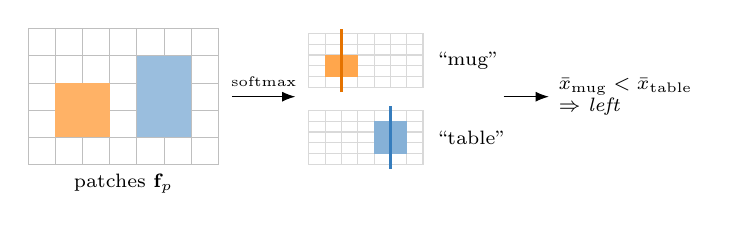
\begin{tikzpicture}[font=\scriptsize, >=Latex, scale=1.15]
  % image grid
  \foreach \i in {0,...,6} \foreach \j in {0,...,4}
    \draw[gray!50] (\i*0.3,\j*0.3) rectangle ++(0.3,0.3);
  \fill[orange!60] (0.3,0.3) rectangle ++(0.6,0.6);
  \fill[cvprblue!50] (1.2,0.3) rectangle ++(0.6,0.9);
  \node[below] at (1.05,0) {patches $\mathbf{f}_p$};
  % arrow
  \draw[->] (2.25,0.75) -- (2.95,0.75) node[midway,above]{\tiny $\mathrm{softmax}$};
  % maps
  \begin{scope}[shift={(3.1,0.85)}]
    \foreach \i in {0,...,6} \foreach \j in {0,...,4}
      \draw[gray!30] (\i*0.18,\j*0.12) rectangle ++(0.18,0.12);
    \fill[orange!70] (0.18,0.12) rectangle ++(0.36,0.24);
    \node[right] at (1.3,0.3) {``mug''};
    \draw[orange!90!black, thick] (0.36,-0.05) -- (0.36,0.65);
  \end{scope}
  \begin{scope}[shift={(3.1,0)}]
    \foreach \i in {0,...,6} \foreach \j in {0,...,4}
      \draw[gray!30] (\i*0.18,\j*0.12) rectangle ++(0.18,0.12);
    \fill[cvprblue!60] (0.72,0.12) rectangle ++(0.36,0.36);
    \node[right] at (1.3,0.3) {``table''};
    \draw[cvprblue, thick] (0.9,-0.05) -- (0.9,0.65);
  \end{scope}
  \draw[->] (5.25,0.75) -- (5.75,0.75);
  \node[align=left, right] at (5.75,0.75) {$\bar{x}_\text{mug} < \bar{x}_\text{table}$\\$\Rightarrow$ \emph{left}};
\end{tikzpicture}
\caption{\textbf{Patch read-out.} Patch features from CLIP's last layer are softly assigned to the two object names; the caption is judged \emph{left} if the subject's mean $x$ position is smaller.}
\label{fig:method}
\end{figure}

\paragraph{Patch features.}
Let $\mathbf{h}_p$ be the token of patch $p$ entering CLIP's last vision block.
Plain last-layer tokens are poorly aligned with text, so I compare two variants:
(i) \emph{plain} output tokens of the last block, and
(ii) the \emph{value path} of the last attention layer as in MaskCLIP~\cite{zhou2022maskclip},
\begin{equation}
\mathbf{f}_p = \mathrm{norm}\big(W_\text{proj}\,\mathrm{LN}_\text{post}\big(W_o W_v\,\mathrm{LN}_1(\mathbf{h}_p)\big)\big),
\end{equation}
both projected into CLIP's joint space with the same post-norm and projection used for the pooled vector.

\paragraph{Decision rule.}
The subject $a$ and object $b$ are parsed from the caption (``A \emph{mug} to the left of a \emph{table}'') and encoded with the prompt ``a photo of a \{name\}.'' as $\mathbf{t}_a, \mathbf{t}_b$.
Each patch is softly assigned to the two names,
$w_{p,k} = \mathrm{softmax}_{k\in\{a,b\}}(\tau\,\mathbf{f}_p\!\cdot\!\mathbf{t}_k)$ with $\tau=100$,
and each name gets a mean horizontal position $\bar{x}_k = \sum_p w_{p,k}x_p / \sum_p w_{p,k}$, with $x_p\in[0,1]$.
The prediction is \emph{left} if $\bar{x}_a < \bar{x}_b$.
For one-object captions (``A dog on the left''), the weights are a softmax over patches of $\tau\,\mathbf{f}_p\!\cdot\!\mathbf{t}_a$ and $\bar{x}_a$ is compared with $0.5$.
Nothing is trained.

\paragraph{Variant selection.}
On the 400 held-out COCO images, plain tokens score 26.5\% (B/32) and 25.5\% (L/14), while the value path scores 73.5\% and 77.3\%.
The value path is therefore used for all test sets, which are run once.

\begin{table*}[t]
\centering
\small
\setlength{\tabcolsep}{4.5pt}
\begin{tabular}{@{}llccccc@{}}
\toprule
Model & Method & What'sUp A & What'sUp B & COCO-spatial 1 & COCO-spatial 2 & What'sUp A pair / same-answer \\
\midrule
\multirow{4}{*}{ViT-B/32}
 & CLIP (zero-shot)              & 49.0 & 52.9 & 50.9 & 48.7 & \phantom{0}1.9 / 94.2 \\
 & Global offset (E3)            & 50.0 & 49.5 & 50.4 & 52.7 & \phantom{0}0.0 / 100 \\
 & Mirror subtraction (E3)       & 49.5 & 49.0 & 52.2 & 52.0 & 17.5 / 64.1 \\
 & \textbf{Patch read-out (E4b)} & \textbf{74.3} & \textbf{99.5} & \textbf{83.7} & \textbf{81.7} & \textbf{50.5} / 47.6 \\
\midrule
\multirow{4}{*}{ViT-L/14}
 & CLIP (zero-shot)              & 48.5 & 52.9 & 51.0 & 47.3 & \phantom{0}1.9 / 93.2 \\
 & Global offset (E3)            & 50.0 & 51.0 & 50.8 & 57.3 & \phantom{0}2.9 / 94.2 \\
 & Mirror subtraction (E3)       & 51.0 & 54.4 & 47.0 & 47.7 & 24.3 / 53.4 \\
 & \textbf{Patch read-out (E4b)} & \textbf{82.5} & \textbf{100.0} & \textbf{90.4} & \textbf{85.7} & \textbf{67.0} / 31.1 \\
\bottomrule
\end{tabular}
\caption{\textbf{Main results.} Left/right accuracy (\%, chance 50). The last column gives pair accuracy (both photos of a What'sUp~A pair correct, chance 25) and the rate of picking the same word for both photos. \emph{Global offset} subtracts the mean score on held-out COCO; \emph{mirror subtraction} is \cref{eq:mirror}. No method in this table is trained.}
\label{tab:main}
\end{table*}

\paragraph{Results.}
\cref{tab:main}: the read-out lifts What'sUp~A from 49.0 to 74.3\% (B/32) and from 48.5 to 82.5\% (L/14), What'sUp~B to 99.5/100\%, and COCO-spatial to 82--90\%.
Pair accuracy on What'sUp~A rises from 1.9\% to 50.5/67.0\%, so the gain is not a shift toward one word.
The larger model is better on every set, and What'sUp~B, with a single large object on a plain table, is solved almost perfectly.
What'sUp~A remains the hardest set; I have not analysed its errors per object pair.

%%%%%%%%%%%%%%%%%%%%%%%%%%%%%%%%%%%%%%%%%%%%%%%%%%%%%%%%%%%%%%%%%%%%%%%%%
\section{Discussion and limitations}
\label{sec:limits}

\paragraph{What the results support.}
Left/right is largely absent from CLIP's pooled image vector and nearly invisible to its text encoder, but is present in the patch features before pooling.
This explains why the fine-tuning in E1/E2 had nothing to work with: the text encoder can only shift its word preference when the image vector does not carry the relation.

\paragraph{Limitations.}
\begin{itemize}
\setlength\itemsep{0pt}
\item The final decision compares $x$ positions of two named objects with a hand-written rule. It covers only left/right, requires both object names, and does not change CLIP's caption matching.
\item The patch features come from MaskCLIP~\cite{zhou2022maskclip}; the contribution here is the diagnosis leading to them and the left/right evaluation.
\item Plain last-layer tokens score clearly \emph{below} chance on held-out COCO (26\%), so they do carry position but the name matching reads it reversed. I did not investigate why.
\item Results cover two OpenAI CLIP models and four test sets; other model families and spatial relations (above/below, front/behind) are untested.
\item E2 unfroze a single block; deeper image-side fine-tuning or training a pooling layer was not tried.
\end{itemize}

\paragraph{Next steps.}
A natural extension is to train only a small position-aware pooling head on top of frozen patch features, so that the information found here is used inside CLIP's own scoring rather than by an external rule, and to test the same read-out for vertical relations.

{
\small
\bibliographystyle{ieeenat_fullname}
\bibliography{refs}
}

\end{document}
